% Title: gl2ps_renderer figure
% Creator: GL2PS 1.4.0, (C) 1999-2017 C. Geuzaine
% For: Octave
% CreationDate: Fri Dec 29 11:24:35 2017
\setlength{\unitlength}{1pt}
\begin{picture}(0,0)
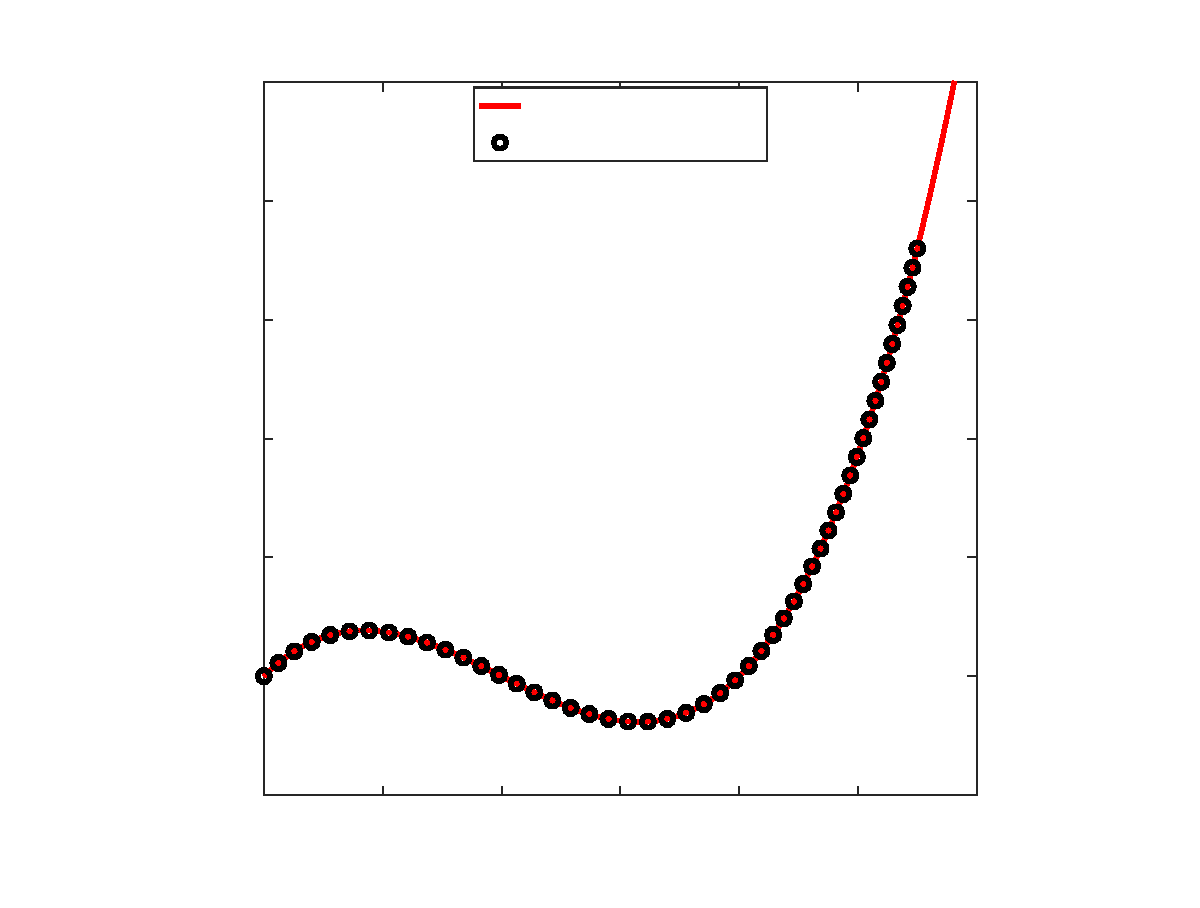
\includegraphics{Fig6Epscargabaja-inc}
\end{picture}%
\begin{picture}(560,420)(0,0)
\fontsize{15}{0}
\selectfont\put(118.65,41.1956){\makebox(0,0)[t]{\textcolor[rgb]{0.15,0.15,0.15}{{0}}}}
\fontsize{15}{0}
\selectfont\put(175.7,41.1956){\makebox(0,0)[t]{\textcolor[rgb]{0.15,0.15,0.15}{{0.5}}}}
\fontsize{15}{0}
\selectfont\put(232.75,41.1956){\makebox(0,0)[t]{\textcolor[rgb]{0.15,0.15,0.15}{{1}}}}
\fontsize{15}{0}
\selectfont\put(289.8,41.1956){\makebox(0,0)[t]{\textcolor[rgb]{0.15,0.15,0.15}{{1.5}}}}
\fontsize{15}{0}
\selectfont\put(346.85,41.1956){\makebox(0,0)[t]{\textcolor[rgb]{0.15,0.15,0.15}{{2}}}}
\fontsize{15}{0}
\selectfont\put(403.9,41.1956){\makebox(0,0)[t]{\textcolor[rgb]{0.15,0.15,0.15}{{2.5}}}}
\fontsize{15}{0}
\selectfont\put(460.95,41.1956){\makebox(0,0)[t]{\textcolor[rgb]{0.15,0.15,0.15}{{3}}}}
\fontsize{15}{0}
\selectfont\put(113.646,46.2){\makebox(0,0)[r]{\textcolor[rgb]{0.15,0.15,0.15}{{-0.5}}}}
\fontsize{15}{0}
\selectfont\put(113.646,103.25){\makebox(0,0)[r]{\textcolor[rgb]{0.15,0.15,0.15}{{0}}}}
\fontsize{15}{0}
\selectfont\put(113.646,160.3){\makebox(0,0)[r]{\textcolor[rgb]{0.15,0.15,0.15}{{0.5}}}}
\fontsize{15}{0}
\selectfont\put(113.646,217.35){\makebox(0,0)[r]{\textcolor[rgb]{0.15,0.15,0.15}{{1}}}}
\fontsize{15}{0}
\selectfont\put(113.646,274.4){\makebox(0,0)[r]{\textcolor[rgb]{0.15,0.15,0.15}{{1.5}}}}
\fontsize{15}{0}
\selectfont\put(113.646,331.45){\makebox(0,0)[r]{\textcolor[rgb]{0.15,0.15,0.15}{{2}}}}
\fontsize{15}{0}
\selectfont\put(113.646,388.5){\makebox(0,0)[r]{\textcolor[rgb]{0.15,0.15,0.15}{{2.5}}}}
\fontsize{14}{0}
\selectfont\put(289.8,23.1956){\makebox(0,0)[t]{\textcolor[rgb]{0.15,0.15,0.15}{{$x$}}}}
\fontsize{14}{0}
\selectfont\put(79.6456,217.35){\rotatebox{90}{\makebox(0,0)[b]{\textcolor[rgb]{0.15,0.15,0.15}{{$\lambda$}}}}}
\fontsize{12}{0}
\selectfont\put(244.634,377){\makebox(0,0)[l]{\textcolor[rgb]{0,0,0}{{Solución Exacta}}}}
\fontsize{12}{0}
\selectfont\put(244.634,359.333){\makebox(0,0)[l]{\textcolor[rgb]{0,0,0}{{Solución Numérica}}}}
\end{picture}
